%!TEX root = ../../thesis_master.tex

%%%%%%%%%%
\chapter{Theoretical Background and State of the Art}
\label{chap:theory-state-art}
%%%%%%%%%%

\section{Visual Servoing Theoretical Basics}
\label{sec:vs-theory}

In this section the theoretical background of visual servo controllers is briefly discussed. The different parts of a Visual Servoing scheme are presented and the basic strategy is illustrated. It is usual in the literature to take \cite{chaumette_visual_2006} and \cite{chaumette_visual_2007} as the main reference when it comes to the theoretical setup of the discipline. As a result, the following description is based on these popular sources\footnote{The interested reader should visit the Lagadic research group home page (\url{http://www.irisa.fr/lagadic}), pioneers in the area.}.

Visual Servoing is defined in the literature as the use of computer vision data to control the motion of a robot. The image data comes from a camera, which can observe the robot fixed in the space or moving with the robot. The latter approach is know as eye-in-hand Visual Servoing and is the selected one for the case of this work.

\nomenclature[ba]{CV}{Computer Vision}

Visual servo controllers accomplish their task of reaching a certain pose by trying to minimize the following error $\bm{e}(t)$

\begin{equation}
\bm{e}(t) = \bm{s}(\bm{m}(t), \bm{a}) - \bm{s}^\ast
\label{eq:vs-th-1}
\end{equation}

Here, $\bm{m}(t)$ is a set of image measurements (e.g. the image coordinates of the interest points or the image centroid of an object), that is, information computed from the image data. With the help of these measurements a vector of $k$ visual features, $\bm{s}(\bm{m}(t), \bm{a})$ is obtained, in which $\bm{a}$ is a vector containing different camera parameters. In contrast, $\bm{s}^\ast$ defines a set of desired features.

For the present case, where the target is not moving,  $\bm{s}^\ast$ and the changes in $\bm{s}$ depend only on the camera motion.

There exist two main variants of Visual Servoing depending on how the features vector $\bm{s}$ is defined. On the one hand, Image Based Visual Servoing (IBVS) takes as $\bm{s}$ a set of features already available within the image data. It can be seen as a control of the features in the image plan such that moving the features to a goal configuration implicitly results in the task being accomplished (see \cite{espiau_1992}). On the other hand, Position Based Visual Servoing (PBVS) considers for $\bm{s}$ a set of 3D parameters that must be estimated from the image data. Once the parameters are available, pose estimation is conducted and the Visual Servoing task results in a cartesian motion planing problem.

\nomenclature[ba]{IBVS}{Image Based Visual Servoing}
\nomenclature[ba]{PBVS}{Position Based Visual Servoing}

Using the PBVS approach leads to the necessity of camera calibration and estimation of the flying robot pose, these are two big disadvantages for the application intended in this work. On the other side, IBVS needs no camera calibration and allows the robot to achieve the pose desired without any pose estimation process. Resulting in a convenient method for cheap systems.

A simple velocity controller can be arranged in the following way. Let $\bm{v}_c = (v_c, \bm{\omega}_c)$ be the spatial velocity of the camera, with $v_c$ the instantaneous linear velocity of the origin of the camera frame and $\bm{\omega}_c$ the instantaneous angular velocity of the camera frame, as a result the temporal variation of the features can be expressed as

\begin{equation}
\dot{\bm{s}} = \bm{L_s} \bm{v}_c
\label{eq:vs-th-2}
\end{equation}

Where $\bm{L_s} \in \mathbb{R}^{k \times 6}$, the feature Jacobian, acts as interaction matrix relating the camera velocity and the change in the visual features.

The time variation of the error to be minimized can be obtained by combining \ref{eq:vs-th-1} and \ref{eq:vs-th-2}

\begin{equation}
\dot{\bm{e}} = \bm{L_e} \bm{v}_c
\label{eq:vs-th-3}
\end{equation}

with $\bm{L_e} = \bm{L_s}$. The input for such a controller is the camera velocity  $\bm{v}_c$, which, using \ref{eq:vs-th-3}, can be set in such a way that an exponential decrease of the error is imposed (i.e. $\dot{\bm{e}} = - \lambda \bm{e}$) 

\begin{equation}
\bm{v}_c = - \lambda \bm{L_e}^+ \bm{e}
\label{eq:vs-th-4}
\end{equation}

Here, $\bm{L_e}^+ \in \mathbb{R}^{k \times 6}$ is the Moore-Penrose pseudoinverse of $\bm{L_e}$. It is computed as $\bm{L_e}^+ = (\bm{L_e}^T \bm{L_e})^{-1} \bm{L_e}^T$, provided that $\bm{L_e}$ is of full rank 6. Imposing this condition leads to $\| \dot{\bm{e}} - \lambda \bm{L_e}^T \bm{L_e} \bm{e} \|$ and $\| \bm{v}_c \|$ being minimal. Note that for the special case of $k=6$, if $\bm{L_e}$ is nonsingular, it is possible to obtain a simpler expression using the matrix inversion $\bm{v}_c = - \lambda \bm{L_e}^{-1} \bm{e}$.

When implementing real systems it is not possible to know perfectly either $\bm{L_e}$ or $\bm{L_e}^{+}$. Thus, an approximation of these two matrices is introduced, noted with the symbol $\widehat{\bm{L_e}}$ for the approximation of the error interaction matrix and $\widehat{\bm{L_e}^+}$ for the approximation of the pseudoinverse of the interaction matrix. Inserting this notation in the control law we obtain

\begin{equation}
\bm{v}_c = - \lambda \widehat{\bm{L_e}^+} \bm{e}
\label{eq:vs-th-5}
\end{equation}

Once the basic appearance of a visual servo controller has being presented, the goal is to ask the following questions: How should $\bm{s}$ be chosen?  What is the form of $\bm{L_s}$? How should we estimate $\widehat{\bm{L_e}^+}$?

In the simplest approach, the vector $\bm{s}$ is selected as a set of image-plane points, where $\bm{m}$ are the set of coordinates of these  image points and $\bm{a}$ the camera intrinsic parameters. Later in this work, a more complex definition for the image features vector $\bm{s}$ will be used.

Concerning the interaction matrix $\bm{L_s}$ 

\subsection*{The Interaction Matrix}

The interaction matrix, which relates the camera velocity to the change of the visual features, is strictly related to the the camera model. A camera model describes the correspondence between objects in 3D space and their appearance in a 2D image. Here, the pinhole camera model is used.

The camera image capture is a procedure which projects a 3D point from its coordinates in the camera frame, $\bm{X} = (X, Y, Z)$, to a 2D image point with coordinates $\bm{x} = (x, y)$. From this geometry we have

\begin{equation}
\begin{cases}
x = X/Z = (u - c_u) / f \alpha \\
y = Y/Z = (v - c_v) / f
\end{cases}
\label{eq:vs-th-6}
\end{equation}

where $\bm{m} = (u, v)$ gives the coordinates of the image point in pixel units, and $\bm{a} = (c_u, c_v, f, \alpha)$ is the set of camera intrinsic parameters: $c_u$ and $c_v$ are the coordinates of the principal point, $f$ is the focal length, and $\alpha$ is the ratio of the pixel dimensions. For a feature point: $\bm{s} = \bm{x} = (x, y)$.

\begin{figure}[ht]
	\centering
	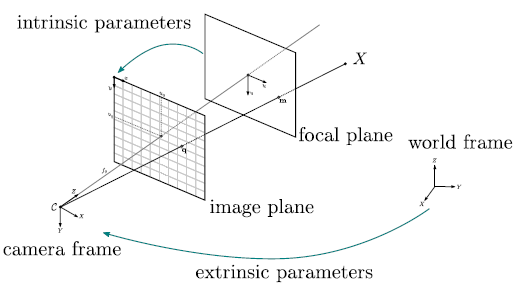
\includegraphics[keepaspectratio, width=9cm]{content/chapter_02/images/pinhole_camera.png}
	\caption{Pinhole camera model}
	\label{fig:pin-hole}
\end{figure}

Taking the time derivative of the projection Equation \ref{eq:vs-th-6}, we obtain

\begin{equation}
\begin{cases}
\dot{x} = \dot{X}/Z - X\dot{Z}/Z^2 = (\dot{X} - x \dot{Z})/Z \\
\dot{y} = \dot{Y}/Z - Y\dot{Z}/Z^2 = (\dot{X} - y \dot{Z})/Z
\end{cases}
\label{eq:vs-th-7}
\end{equation}

The velocity of the 3D point can be related to the spatial velocity of the camera using the equation for the velocity in a non-inertial reference frame

\begin{equation}
\dot{\bm{X}} = - \bm{v}_c - \omega_c \times \bm{X} \Leftrightarrow
\begin{cases}
\dot{X} = - v_x - \omega_y Z + \omega_z Y \\
\dot{Y} = - v_y - \omega_z X + \omega_x Z \\
\dot{Z} = - v_z - \omega_x Y + \omega_y X 
\end{cases}
\label{eq:vs-th-8}
\end{equation}

Introducing \ref{eq:vs-th-8} in \ref{eq:vs-th-7} and grouping terms, it can be written

\begin{equation}
\begin{cases}
\dot{x} = - v_x / Z + x v_z / Z + xy \omega_z - (1 + x^2) \omega_y + y \omega_z \\
\dot{y} = - v_y / Z + y v_z / Z + xy \omega_z - (1 + y^2) \omega_x + x \omega_z 
\end{cases}
\label{eq:vs-th-9}
\end{equation}

using matrix notation

\begin{equation}
\dot{\bm{x}} = \bm{L_x} \bm{v}_c
\label{eq:vs-th-10}
\end{equation}

where the interaction matrix that relates the camera velocity $\bm{v}_c$ to the velocity of the image point $\dot{\bm{x}}$ is

\begin{equation}
\bm{L_x} = 
\begin{bmatrix}
\frac{-1}{Z} & 0  & \frac{x}{Z}  & xy  &  -(1+x^2) & y \\ 
0 & \frac{-1}{Z} &  \frac{y}{Z} & 1+y^2 &  -xy & -x
\end{bmatrix}
\label{eq:vs-th-11}
\end{equation}

In Equation \ref{eq:vs-th-11}, the value $Z$ corresponds to the depth of the point relative to the camera frame. As a result, any Visual Servoing scheme using this form of the interaction matrix must provide an estimation of this value. Furthermore, the camera intrinsic parameters are necessary to compute $x$ and $y$. Therefore, it is not possible to use directly $\bm{L_x}$, but an approximation $\widehat{\bm{L_x}}$ is to be used.

\subsection*{Approximation of the Interaction Matrix}

When the current depth $Z$ of each point is known, there is no need of approximation and $\widehat{\bm{L_e}^+} = \bm{L_e}^+$ for $\bm{L_e} = \bm{L_x}$ can be used. However, this approach requires the estimation of $Z$ for all iterations of the scheme control (see \cite{hutchinson_1996}), which may be conducted by means of pose estimation methods.

A second alternative is to use $\widehat{\bm{L_e}^+} = \bm{L_{e^\ast}}^+$, where $\bm{L_{e^\ast}}$ is the value of $\bm{L_{e}}$ for the desired position ($\bm{e} = \bm{e}^\ast = 0$) (see \cite{espiau_1992}). Here, the depth parameter only needs to be estimated once for every point.

\subsection{Pinhole Camera Model}

The basic idea of a photographic camera is placing a film in front of an object so it records the reflected light on this object, obtaining a representation of the object thanks to the projection of each of the points of the object into the film.

Instead of placing just the film, a barrier is placed between it and the object leaving only a small opening (pinhole) so it blocks most of the rays reducing blurring. This small hole on the barrier is called aperture. The aperture acts as the center of the camera and the distance between the image plane (the film) and the pinhole is known as focal length.

The image formation is driven by the projective geometry. In this kind of geometry, straight lines are also straight in the image and the parallel lines in the 3D space world intersect in the image at the so-called vanishing point.
 
\subsection{Image Moments as Visual Features}
\label{sec:image-moments}

As in other computer vision problems, the choice of visual features has a strong influence on the performance of an visual servo controller. An image feature is a piece of information extracted from an image and may be helpful to solve a certain task. Depending on the problem, different kind of features can be interesting for the user. These features are a specific structure in the image such as points, edges or closed contours, which are detected by means of operations on their pixel neighborhood.

Usually, the desired characteristics \cite{Szeliski2011} for a visual feature are: locality (robust to occlusion and cluttering), invariance to transformations such as rotation or scaling, robustness against noise or compression and efficiency (so they can be computed in real-time). In addition to that, for a visual servoing task it is convenient that the set of features is decoupled, so it can be used to control independently all the degrees of freedom of the robot.

Image moments are the result of a particular weighted average of the pixels' intensities of an image or a combination of various of these moments. They are useful to describe an object after segmentation, and have been used in computer vision for patter-recognition tasks \cite{hu_1962}.

Before the introduction of image moments, other visual features such as points from corner detectors, Fourier descriptors or light intensity where used to carry visual servoing tasks. Image moments result of particular interest for planar objects when the desired configuration is such that the camera plane and the object are parallel. They are easy to compute, robust to noise and its interaction matrix can be computed for any case thanks to the analytical method presented in \cite{chaumette_image_2004}. The inclusion of spherical image moments as visual features has the advantage that they are invariant under rotation of the camera frame \cite{bourquardez_stability_2006}. 

Image moments have also the advantage of being intuitive for simple cases. The simplest example of image moments are the area and centroid coordinates of an object.

For a greyscale image with pixel intensities $I(x, y)$, the raw image moments $m_{ij}$ are computed as

\begin{equation}
m_{ij} = \sum_{k=1}^n x_k^i y_k^j
\end{equation}

While entered moments are given by

\begin{equation}
\mu _{ij} = \sum_{k=1}^n \left( x_k - x_g \right)^i \left( y_k - y_g \right)^j
\end{equation}

Where for the area $a = m_{00}$ and for the centroid coordinates $\left\lbrace \bar{x_g}, \bar{y_g} \right\rbrace = \left\lbrace m_{10}/m_{00}, m_{01}/m_{00} \right\rbrace $. Any moment defined in this way, is known to be invariant to 2D translational motion. 

Several works \cite{bourquardez_2009} \cite{tahri_2005} introduced the area and centroid coordinates of a target as visual features. For this case, the interaction matrix has the following form \cite{tahri_2005}.

\begin{equation}
\bm{L}_{x_g} = \begin{bmatrix} -C & 0 & C x_g & \varepsilon_1 & -(1+\varepsilon_2) & y_g \end{bmatrix}
\end{equation}

In this work, the normalized area and normalized centroid coordinates of a planar target are used as visual features. 

\subsection{Robot Operating System (ROS)}

The Robot Operating System (ROS)\footnote{\url{www.ros.org}} is an open-source, operating system for robots. It provides all the capabilities expected from any operating system, including hardware abstraction, low-level device control, implementation of commonly-used functionalities, message-passing between processes and package management \cite{ROS_Intro}.

ROS works as a peer-to-peer network of processes, called \emph{nodes}, connected through the ROS communication infrastructure. ROS implements several communication interfaces such as \emph{services}, \emph{topics} and a \emph{Parameter Server}.

As a result, ROS works as a framework where the user can implement the desired robotic system modularly as a graph connecting several independent processes. The main ROS concepts are \cite{ROS_Concepts}:

\begin{itemize}
	\item \emph{Nodes}: Nodes are processes that perform a certain computation. The robotic system is decomposed in functionalities running in each of the in different nodes. For example, one node processes de camera information, other node controls the wheel motors and a third node is responsible of the path planning.
	
	\item \emph{Master}:The ROS Master builds and maintains the name registration and lookup of the rest of components of the computation graph, so it allows the identification between nodes to establish the desired communication.
	
	\item \emph{Messages}: Messages are the data transfered between nodes. A message is a data structure comprising typed fields. The standard primitive types (integer, float point, boolean, etc.) can be combined in nested structures or arrays.
	
	\item \emph{Topics}: Topics are an asynchronous streaming of data between nodes following a publish/subscribe semantic. For example, data coming from a sensor. A node can send out a message through a topic publishing into it and an interested node can receive the message by subscribing the topic. A topic can use only a unique type of message. Topics work as an abstraction layer to separate the data production from the data manipulation using different nodes that communicate between each other without depending one on the other.
	
	\item \emph{Services}: A constant stream of data is not always the desired communication case. It is also possible to desire a request/reply interaction between to nodes. For example to start the motors of a robot. This kind of communication is conducted using services. A providing node offers a service under a name and a client uses the service by sending the request message and awaiting the reply.
	
	\item \emph{Parameter Server}: The Parameter Server allows data to be stored in a centralized data structure similar to a dictionary, where it can be accessed by any node. 
\end{itemize}

In the present work, the system designed works as a set of nodes establishing communication between the \emph{action interface} described in the Section TODO, which subscribe to the sensor topics of the robot and publish control command to the command topic of the robot.

\section{State of the Art}

\subsection{Visual Servoing for Aerial Robots}

In this section, the literature on the use of Visual Servoing to control de translation and yaw motion of aerial robots is analyzed. The focus of this review is on the IBVS approach, where image feature errors between the current and target image are mapped to actuator inputs through the inverse of the Jacobian matrix. The different approaches presented complete the basic IBVS formulation with alternatives on feature selection, Jacobian matrix construction and different control strategies to make the error converge to zero, and with it, the relative pose between UAV and target object will converge to the desired one.

The task is to move the camera attached quadrotor to match the observed image features with the predefined desired image features obtained from a stationary object.

In \cite{ceren_vision-based_2009}, the visual servo controller presented is very simple, using feature points and a simple proportional law to control the kinematics of the robot. The VS technique is not explained in detail since it uses the MATLAB Visual Servoing Toolbox\footnote{\url{https://sourceforge.net/projects/vstoolbox/}}. However, the paper is a good reference when it comes to the system description of the most simple approach to follow for the control of a quadrotor using visual servoing: The desired velocities on the image plane are computed with the visual information, transformed to the robot body frame and later to motor speeds that provide the robot with this motion. In this case, a PD controller is used to make the robot follow the chosen velocities. 

\nomenclature[ba]{PD}{Proportional Derivative}

The Visual Servoing research was originally developed for serial manipulators. In order to translate these techniques to aerial robots there are different aspects that may be considered, derived of the fact that a quadrotor is an under-actuated system:

\begin{itemize}
	\item Feature depth estimation.
	\item Dynamics of the system leading to a high coupling between camera motion and target (visual feature) motion on the image plane.
\end{itemize}

To cope with these problems different solutions have been proposed and applied for the usual configuration of a quadrotor helicopter, with the camera mounted on its platform (eye-in-hand configuration).

 In the past, several approaches have been taken to face the problem of depth estimation, such as: partial pose estimation (see \cite{malis_2_1999}), adaptive control (see \cite{Papanikolopoulos}) or estimation of the Jacobian using quasi-Newton methods (see \cite{Piepmeier}). Nowadays, the most frequent approach is the use of a partitioned control that allows the uncoupling of translational and rotational degrees of freedom\footnote{However, it is important to bear in mind that due to the under-actuated dynamics of an usual 4 DOF quadrotor, it is only possible to control the three linear velocities and the yaw (rotational) speed. While the other two rotational speeds, roll and pith, are used to move the thrust vectors of the propellers and thus generate movement on the horizontal plane.}.
 
 \cite{hamel_2002} is one of the pioneering works to cope with the visual servo control of under-actuated systems as a quadrotor. Introduces the idea of controlling the full dynamics of the vehicle. The approach requires separate measurements of linear and angular velocities which are not needed in classical IBVS, since for this case the kinematic velocities are used directly as control variables. In particular the method presented, needs only a single inertial direction. For the case of quadrotors, which usually require hovering applications, this is the vertical axis acceleration, provided by a filtered IMU signal. Due to the rotational ego-motion of the camera, the dynamics of the image point involve the angular velocity as well as the velocity linear velocity of the vehicle. This dependence destroys the explicit triangular cascade structure of rigid body motion expressed in the inertial frame. However, under certain conditions on the camera geometry, it is possible to recover a passivity-like property (from virtual input to the backstepping error) sufficient to apply a backstepping control design for the non-linear dynamical system. The paper the formulates that only image geometry that preserves the passivity-like properties of the body fixed frame dynamics of a rigid object in the image space are those of a spherical camera. Thus, introducing the use of spherical image moments\footnote{To use spherical moments is not necessary to implement physically a spherical camera, just to compute numerically the spherical moments of the image.}.

For serial manipulators, a low-level actuator is usually employed to compensate the dynamic behavior of the system, making possible to control it with velocity commands as a first order system. For a full-dynamics quadrotor model accounting for aggressive maneuvers this is not at all the case, since it is a fourth order system. Thus, other strategies are usually considered to control such a robot (see \cite{Mellinger} for a comprehensive description of the control of the dynamics of a quadrotor and its trajectory generation in space). Already in the basic literature on Visual Servoing (see \cite{chaumette_visual_2007}) the authors suggest that kinematic control may not be enough for the case of aggressive maneuvers. 

Image moments are invariant to some transformations like scale, 2D translation or 2D rotation. This has been intensively used in pattern recognition. Introducing visual features based on image moments allows to design a decoupled control scheme when the object is parallel to the image plane (see \cite{tahri_2005}). Later, it is possible to generalize this property for the case of a non-parallel position with respect to the image plane.

% \cite{guenard_2008}

In the work \cite{guenard_2008}, a IBVS controller for the full dynamics of a quadrotor system around the hovering position is proposed. The biggest difficulty to develop dynamic controllers based on IBVS is the high coupling in the image Jacobian between the rotational and translational dynamics. Something that does not happen in the case of PBVS. The paper introduces a new visual error formulation to improve the conditioning of the Jacobian matrix, following the idea of \cite{hamel_2002}. Image moment features are augmented with the information provided by the IMU and used in conjunction with a non-linear controller.

% \cite{bourquardez_2009}

Common strategy is to use to different loops to separate the control problem. The inner attitude loop runs at high gain using IMU measurements, while the outer loop runs at low gain with the visual input of the camera taking care of translation. The visual servo controller (outer loop) provides the attitude control (inner loop) the desired targets and outer loop ensures the stability of the system. An advantage of this approach is the possibility of reuse the IBVS scheme in other platforms since the low-level control of the specific material equipment of the aerial robot is not involved in it.

The paper \cite{bourquardez_2009} focuses in the design of kinematic controllers. The use of zero and first-order image moments as visual features is considered inappropriate for aggressive maneuvers due to its lack of robustness for this case, where Global Asymptotic Stability (GAS) cannot be guaranteed. For this reason, first-order spherical moments are introduced. Different control schemes are proposed in the paper. First, one controller using perspective projections is able of regulating the translation of the system thanks to the decoupled relationship between image and task space obtained. For the case of the camera image plane being parallel to the target plane, it is possible to control the translation of the robot independently of its rotation in a way equivalent to PBVS but without any pose estimation involved. The target depth is introduced as an initial data, so no depth estimation is performed. The strategy is easy to implement and provides a good result within the assumed geometrical limitation.

  \nomenclature[ba]{GAS}{Global Asymptotic Stability}

To overcome the limitations of the simple model presented, the work introduces order control schemes that include spherical projections as visual features and non-linear control techniques that improve the behavior for the case of aggressive maneuvers, although still around the hovering position.
 
 % \cite{ceren_image_2012}

 In \cite{ceren_image_2012}, present two kinematic controllers, one based on points as visual features for IBVS and other implementing a Hybrid Visual Servoing scheme that requires partial pose estimation.
  
  % \cite{jabbari_dynamic_2012}
  
  \cite{jabbari_dynamic_2012} designs a controller for the dynamics of a quadrotor within the IBVS approach. Although spherical moments are able to guarantee GAS, they generate trajectories that are not adequate when transforming to Cartesian coordinates.  In this work, the method presented allows creating trajectories that are not only convenient in the image plane (i.e. where a usual IBVS controller is considered) but also in the Cartesian space. A projection of the perspective image moment features. augmented with inertial information to better control the dynamics, on a virtual plane dependent on the pitch and roll of the robot is proposed. Thus, the paper extends the approach followed in \cite{bourquardez_2009}, here perspective projection was considered useful for a flight perpendicular to the target, but replaced by spherical moments to provide the GAS that it was not able to provide. In this way, a decoupled linear link between image and Cartesian coordinates is obtained using perspective image moments for the case in which the robot does not navigate perpendicular to the target. Finally a non-linear controller is derived for the system.
   
 % \cite{asl_vision-based_2015}
 
 The authors in \cite{asl_vision-based_2015}, propose two improvements to the work presented in the previous paragraph. For most of the controllers in the literature the camera velocity is required. This comes usually from IMU estimations, but due to the usual lack of GPS of the robots the noisy measurements of the IMU may not be enough. The paper proposed a visual flow and non-linear observer strategy to overcome this inconvenience. Secondly, in the standard formulation of the Jacobian matrix a estimation of the visual feature depth is necessary, something which is expensive to include in the controller. This is usually solved tanks to the use of image moments and a predefined target depth. The authors include here a controller to deal with this uncertainty. 
 
   \nomenclature[ba]{GPS}{Global Positioning System}
   

\subsection{Visual Servoing for Aerial Manipulators}

In this section a perspective of Visual Servoing applied to aerial manipulators is presented. The main available literature is analyzed and the common approaches followed in it highlighted. An the end of the section, Table \ref{vs-manipulators-table} summarizes the strategies commented with regard to the main characteristics of each method. 

% Aerial gripping

Some publications related to the University of Pennsylvania GRASP Laboratory\footnote{\url{https://www.grasp.upenn.edu}}  (see \cite{thomas_toward_2014} and \cite{thomas_visual_2016}) have studied the vision-based localization and servoing of quadrotors in grasping and perching tasks. However, the emphasis of these publications lays on the generation of dynamically-feasible trajectories in the image space, thus second order system control is performed instead of the most common kinematic control strategy. These vehicles are not manipulators in the sense of the rest of the approaches presented in this section, since the main task here is hanging from structures and grasping targets by means of aggressive, thus dynamical, maneuvers. In addition to that, the actuator used is not a high-DOF serial manipulator, but a 1 DOF gripper.  

In the last years, a concrete aerial manipulator architecture has been popularized, for example in the context of the European projects ARCAS\footnote{\url{http://www.arcas-project.eu}} and AEROARMS\footnote{\url{http://www.arcas-project.eu}}. These aerial manipulators have usually the task of collecting an structural element from its initial position and fly it to a final position, where the element is used to assemble a strut structure. The main configuration of such a robot is an under-actuated rotary-wing aircraft (usually a quadrotor) and a robotic serial manipulator arm. Different degrees of freedom (DOF) are used for the arm and different camera placements are considered.
 
  \nomenclature[ba]{DOF}{Degree of Freedom}
 
 The usual implementation considers the simultaneous control (at the velocity level) of the mobile platform (i.e. quadrotor) and the manipulator for such a grasping task. Since the sum of the 4 DOF of a quadrotor plus the multiple-DOF of a serial manipulator leads to a redundant system, the possibility of choosing degrees of freedom is used to realize different subtasks (e.g. joint limit reaching prevention). The Visual Servoing controller chosen generates velocity inputs both for the manipulator joints (i.e. $\bm{\dot{q}}$) and for the quadrotor (i.e. translational velocity $\bm{v}$ and rotational velocity $\omega_z$). The use of a weighted pseudo-inverse allows to favor the control of the mobile platform when the distances to the target are bigger and increase the manipulator mobility when it is close to the target.
 
 % \cite{mebarki_image-based_2014}
 
 \cite{mebarki_image-based_2014} propose a quadrotor equipped with a 5 DOF arm. Traditional Visual Servoing distinguishes between two different classes of camera configuration: eye-to-hand (fixed in the workspace) and eye-on-hand (mounted on the mobile platform). In this paper a new configuration for the camera is presented, called onboard-eye-to-hand, i.e. the camera is placed on-board of the robot while it observes the manipulator. In this way, the manipulator can accomplish large rotations while the target is not left out of the camera field of view, as happens in the eye-in-hand configuration. Furthermore, for the case of eye-in-hand configuration, during assembly tasks the manipulator end-effector can contact or impact with objects and damage or obstruct the camera. Thanks to the onboard-eye-to-hand camera configuration the paper is able to introduce a variation of the IBVS approach, called Self Visual Servoing (SVS). Where the error nullified comes directly form the image itself (hence the adjective self) an there is no need for a target image. The servo controller implemented has two different tasks. The main task is positioning the feature points at a target position on the target object and the second one the end-effector motion. The error formulation decouples both tasks and a weighted pseudo-inverse is used to provide a different gain for the arm joints rates $\bm{\dot{q}}$ than for the UAV velocities $\bm{v}$ and $\omega_z$ control.
 
 \nomenclature[ba]{SVS}{Self Visual Servoing}
 
 % \cite{mebarki_exploiting_2013}
 % \cite{mebarki_cross-coupled_2014}
 
Image moments as features for the Visual Servoing are proposed in \cite{mebarki_exploiting_2013} for the previous system. Furthermore, aerial manipulators have to cope with the change of the center of mass during flight due to the effect of suspended loads (see \cite{palunko_2012}). To achieve this behavior, low-level attitude controllers are usually designed to compensate this effects using Cartesian impedance control (see \cite{lippiello_impedance_2012}) or an adaptive control approach is followed. In this case, the system includes a controller to reduce dynamic effects by vertically aligning the arm center of gravity to the multirotor gravitational vector, along with one that keeps the arm close to a desired configuration of high manipulability and avoiding arm joint limits. In \cite{mebarki_cross-coupled_2014}, the author completes the robot with a nonlinear low-level controller that thanks to a integral  approach allows the inclusion of the dynamic coupling of the UAV and the robotic arm, while the control of the system through the velocities provided by the IBVS high-level is maintained.
 
% \cite{danko_evaluation_2014}

In this case the source (see \cite{danko_evaluation_2014}) includes as host a gantry used to emulate an UAV and a 6 DOF manipulator with an end-effector mounted camera (i.e. eye-in-hand). Coordination of redundant degrees of freedom by means of partitioned control. Visual servoing is used to drive the end-effector pose relative to a target thanks to the use of feature points and their desired positions.

% \cite{lippiello_hybrid_2016}
% Uses Gazebo for simulations

\cite{lippiello_hybrid_2016} uses a hybrid-control framework to take advantage of the main benefits of both IBVS and PBVS schemes to control a octorotor with a 6 DOF arm. Kinematic redundancy of the end-effector is used to accomplish secondary tasks and lead by a hierarchical task-composition algorithm, in conjunction with a smooth activation mechanism for the tasks.

% \cite{laiacker_high_2016}


DLR's work within ARCAS project (see \cite{laiacker_high_2016}) uses of an helicopter and a 7 DOF manipulator. The helicopter is a bigger robot when compared to the rest of the systems, with more than 1 m from manipulator to center of gravity. Influence of the arm movement is significant to the helicopter flight and is actively compensated by the robot controller by means of a coordinated control of both elements. The paper discusses performance and accuracy in aerial manipulation, where the time it takes between the measurement of a position difference and its compensation using the manipulator or the flying platform is the main factor. Additionally, the work presents a multi-marker approach to compensate the possible occlusion of the target marker by the manipulator derived of the onboard-eye-to-hand camera configuration.


% \cite{kim_vision-guided_2016}
% (TODO: \cite{kim_vision-guided_2016} contains signal flow char for image processing and IBVS)

A combination of kinematic and dynamic models to develop a passivity-based adaptive controller which can be applied on both position and velocity control is proposed in \cite{kim_vision-guided_2016}. Position control is used for waypoint tracking and landing, while velocity control is triggered for target servoing. The robot is a quadrotor with a 3 DOF arm and an eye-in-hand camera. The work uses IBVS with image moments as visual features and tries to solve two problems of the method when applied to aerial manipulators (under-actuated system). Firstly, movements of the manipulator produce movement of the camera, thus making probable that the target object is taken out of its field of view. For this reason a fisheye camera is used, so it is possible to introduce a bigger field of view. Secondly, the under-actuation of the robot is corrected introducing a image modification method. Velocity weighting of the Jacobian matrix in accordance of the situation is used for the simultaneous control of UAV and manipulator.

% \cite{santamaria-navarro_uncalibrated_2017}

In \cite{santamaria-navarro_uncalibrated_2017}, redundant manipulation and hierarchical control law are combined with a new variation of the IBVS that does not need the camera parameters. The system establishes as primary task the avoidance of obstacles, as well as several secondary tasks. The visual servo strategy is used to drive the arm end-effector to a desired position and orientation by using a camera attached to it. The configuration used is a 4 DOF quadrotor, which is equipped with a 6 DOF robotic arm. In the common IBVS approaches, Jacobian or interaction matrix, which relates the camera velocity with the image feature velocities, depends on a priori knowledge of the intrinsic camera parameters. The paper presents a variation of IBVS called Uncalibrated IBVS, the approach uses the barycenter of the features as control points. The method recovers the coordinates of these control points and also the camera focal length, with this data a new formulation of the Jacobian is constructed. The system also compensates by means of a hierarchical algorithm the position of the manipulator. The implementation of this method withing the ARCAS project uses Gazebo and is available on the Internet under the name Kinton\footnote{\url{https://devel.iri.upc.edu/pub/labrobotica/ros/iri-ros-pkg_hydro/metapackages/iri_visual_servo/}}.

\renewcommand{\tabularxcolumn}[1]{>{\scriptsize}m{#1}}
\newcolumntype{C}{>{\Centering\arraybackslash}X} % centered "X" column
\newcolumntype{B}{>{\hsize=0.8\hsize}C}
\newcolumntype{P}{>{\hsize=0.45\hsize}C}

\begin{sidewaystable}
\setlength\extrarowheight{0.3pt} % for a bit of visual "breathing space"
	%\tiny
	%\scriptsize
	%\footnotesize
	%\small
	\begin{tabularx}{\textwidth}{CPPBPCC}
		\toprule
		\textbf{Reference} & \textbf{Vehicle} & \textbf{Arm's DOF} & \textbf{Camera Configuration} & \textbf{VS Type} & \textbf{Visual feature} & \textbf{Comment} \\ 
		\midrule
		\cite{thomas_toward_2014} and \cite{thomas_visual_2016} & quadrotor  & 1 & eye-in-hand & IBVS & cylinder parameters & agressive maneuvers \\ 
		\cite{mebarki_image-based_2014} & quadrotor  & 5 & onboard-eye-to-hand  & SVS & points (no target) & - \\ 
		\cite{mebarki_exploiting_2013}  & quadrotor  & 5 & onboard-eye-to-hand  & SVS & perspective projection image moments (no target) & - \\ 
		\cite{mebarki_cross-coupled_2014} & quadrotor  & 5 & onboard-eye-to-hand  & SVS & points (no target) & low-lever controller for dynamic coupling robot-arm \\ 
		\cite{danko_evaluation_2014} & grantry & 6 & eye-in-hand & IBVS & points & gantry used to emulate an UAV \\ 
		\cite{lippiello_hybrid_2016} & octortor & 6 & onboard-eye-to-hand  & Hybrid VS & points & hierarchical task-composition algorithm, smooth task activation \\
		\cite{laiacker_high_2016} & helicopter & 7 & onboard-eye-to-hand  & IBVS & points & discusses performance and accuracy, multi-marker approach \\ 
		\cite{kim_vision-guided_2016} & quadrotor  & 3 & eye-in-hand & IBVS  & corrected perspective projection image moments & adaptive controller for both position and velocity, fisheye camera \\ 
		\cite{santamaria-navarro_uncalibrated_2017} & quadrotor  & 6 & eye-in-hand & Uncalibrated IBVS & blobs' barycenters & hierarchical task-composition algorithm \\
		\bottomrule
	\end{tabularx}
	\caption{Overview of the different approaches for VS in flying manipulators}
	\label{vs-manipulators-table}
\end{sidewaystable}
